\documentclass[11pt]{jarticle}

\usepackage[dvipdfmx]{graphicx}

\setlength{\oddsidemargin}{-6.35mm}
\setlength{\textwidth}{171.9mm}

\begin{document}

\title{画像処理実験 第6回}
\author{09430509\\今田将也}
\date{\number\year 年\number\month 月\number\day 日}
\maketitle

\section{greedy.c を完成させ,第1画像の第 i 特徴点と,第2画像の第 j 特徴点の類似度(下記の値)を全てのi,jの組について計算し,行列の(i,j)要素に格納した表を作りなさい}
結果
\tiny
\begin{verbatim}
    53 124   5  59  41  55  72  53  54 116  92  63  85  35 108 101  40  61  52  83  76  56  56  53  67  69  64  57  47  92 
    66 112  38  41  59  47  56  45  54  75 102  65  84  52 100  82  50  57  51  63  70  48  50  53  56  60  55  49  44  99 
    83 120  83  83  78  77  68  43  88  63 115  78 108  74  95  46  80  56  41  61  80  49  86  62  69  50  72  79  76  99 
    43  88  51  67   9  63  61  49  32  90 101  40  66  43  92  74  44  62  45  52  54  39  42  43  54  69  61  46  35 108 
    13  96  54  69  45  85  80  59  63 121 122  52  97  54 112  96  54  68  55  68  67  56  66  63  59  91  71  58  45 103 
    76 134  32  57  49  27  50  54  48  97 115  77  95  53 119  93  59  57  62  68  83  55  58  63  64  61  64  55  56 121 
    59 117  38  42  45  40  52  49  43  81  90  57  74  43  94  70  47  51  46  61  65  41  43  40  56  57  46  42  40  94 
    82 114  55  57  65  30  34  46  58  76 103  66  90  57  91  69  63  45  44  64  69  49  55  49  61  44  46  58  56 116 
   115  98 101  81  95  75  66  47  90  21  94  79  83  90  71  26  85  41  46  71  76  63  69  58  64  29  50  60  80  89 
    78  76  68  60  64  49  38  28  57  39  86  53  56  75  61  39  62  39  43  50  54  49  46  52  53  36  34  33  47  73 
    60 119  52  58  32  47  59  46   3  90 121  63  71  46 121  76  62  60  59  53  65  45  45  63  62  70  57  41  48 129 
    62  94  55  67  60  63  51  28  67  57  51  47  59  44  48  36  47  35  15  72  59  31  54  28  52  32  33  51  52  61 
    57  54  65  55  45  78  65  52  64  70  64   4  43  51  56  68  37  53  40  57  34  49  28  36  43  54  35  32  27  62 
   124 102 102 102 111  97  76  70 135  66  41  65  68  98  14  63  75  67  51 120  83  78  74  44  70  46  47  81  80  56 
    61  93  54  58  59  44  38  39  59  67  72  44  62  45  72  44  49  11  29  57  56  41  53  35  45  33  36  37  47  85 
    56 135  36  63  51  52  61  46  51  95  80  56  75   9  91  76  46  46  32  76  70  32  61  38  55  57  48  59  55 102 
   106 100  98  90  88  85  68  47  85  46  76  70  71  92  58   3  77  41  47  81  81  63  71  49  72  38  48  51  77  72 
   138 137  94 108 121 124 111  97 140 105  22  79  69  94  44  91  74  83  60 163 111  96  77  48  95  71  67  92  92  48 
    55  88  37  61  46  61  62  47  60  96  67  36  56  39  74  77   6  54  35  76  53  50  40  32  52  62  49  45  37  65 
    65 109  56  66  49  48  50  35  53  68  83  57  82  45  67  50  62  43  27  70  67  12  59  42  44  47  44  51  53 104 
    58  63  83  69  54  68  63  46  56  72 160  61  87  78 129  79  74  58  66  10  42  62  57  80  55  64  69  50  43 129 
   103  74  89  75  75  94  80  66  81  64  66  49   6  77  61  68  61  65  59  83  58  81  48  56  71  49  39  46  55  58 
    60  50  80  52  51  78  71  56  66  73 114  36  58  61  91  81  49  64  49  38   1  56  41  61  53  62  58  41  28  89 
    62  86  57  42  62  58  53  44  76  62  74  44  69  39  52  71  45  49  28  65  41  32  47  37  33  41  38  55  40  76 
    39 116  46  62  34  55  56  43  44 102  92  42  76  31  88  75  45  50  27  65  55  30  55  38  59  62  50  50  43 113 
    54  57  52  29  48  54  63  55  48  68 101  39  55  54  91  86  43  56  56  37  29  50  26  56  31  60  50  28  16  85 
    92  88  73  69  78  59  49  35  78  31  68  58  57  65  49  35  64  28  30  64  59  51  59  43  54   5  32  52  65  65 
    59  74  64  46  48  56  44  39  53  62  78  30  49  39  58  56  44  50  32  47  29  33  38  34  45  42  26  34  31  84 
    95  63  90  63  80  87  77  54  81  33  62  55  43  84  53  34  67  52  49  65  57  64  43  48  49  37  45  44  52  42 
    70  70  58  60  48  78  71  48  55  55  63  33  39  53  70  45  40  36  40  55  52  54  32  30  52  38  36  26  39  56 
\end{verbatim}
\normalsize

\section{上記の条件(i)–(iii)の意味を考察しなさい.}
(i)(ii) 画像1に対して画像2の特徴点が複数選ばれないことを意味している.
(iii) 画像1と画像2の特徴点の類似度が高いということを意味している

\section{方法1の問題点}
\begin{itemize}
    \item SSDの和が方法2と比べて大きいので精度がよくない.
    \item もし対応する特徴点が二枚目の画像にないときはすごく異なる対応点が選ばれてしまう.
    \item 同じ列に選ばれた点よりもとても強い特徴点がいても選ばれないことがある.
  \end{itemize}

\section{方法2の問題点}
\begin{itemize}
    \item 方法1同様,もし対応する特徴点が二枚目の画像にないときはすごく異なる対応点が選ばれてしまう.
    \item INFINITYで上書きしたものは本当にいらないものなのかどうかの判断ができていない.
  \end{itemize}

\section{greedy.cに追加し,動作させなさい.また,これをもとに方法2を完成させなさい}
以下が方法2のソースコードである.点の数だけ対応を見つける際に,各行,各列の最小値を見つけて,かぶらないようにその点の
横と縦を見ないようにする動作をシている.
\begin{verbatim}
    int matchMethod2(double w[][4],Matrix*mt,Image*im ,
    int x1[][2],int N1,Image*im2,int x2[][2],int N2){
  int i,j,k,l,n = 0;
  int minElem[3] = {0,0,INFINITY_INT};
  // SSDの表中の最小値
  for(i=0;i<MAX;i++){//点の数
    for(j=0;j<mt->W;j++){//横幅
      for(k=0;k<mt->H;k++){//縦幅
        if(Elem(mt,j,k) < minElem[2]){
          minElem[0] = j;
          minElem[1] = k;
          minElem[2] = (int)Elem(mt,j,k);
          //printf("%d,%d,%d\n",minElem[0],minElem[1],minElem[2]);
        }
      }
    }
    for(k=0;k<MAX;k++) Elem(mt,minElem[0],k)=INFINITY_INT;//横固定
    for(k=0;k<MAX;k++) Elem(mt,k,minElem[1])=INFINITY_INT;//縦固定
    //MatrixPrint(mt);
    printf("%d,%d,%d,%d,\n",x1[minElem[0]][0],x1[minElem[0]][1],
    x2[minElem[1]][0],x2[minElem[1]][1]);
    w[n][0] = x1[minElem[0]][0];
    w[n][1] = x1[minElem[0]][1];
    w[n][2] = x2[minElem[1]][0];
    w[n][3] = x2[minElem[1]][1];
    n++;
    minElem[2]=INFINITY_INT;
  }
  return n;
}
\end{verbatim}
\section{4組の特徴点対を選び,射影変換行列を計算し,合成画像を作成しなさい.}
算出した特徴点
\begin{verbatim}
    315,495,564,507,
    259,538,507,548,
    119,196,367,211,
    142,517,393,522,
\end{verbatim}
    \begin{figure}[ht]
        \centering
        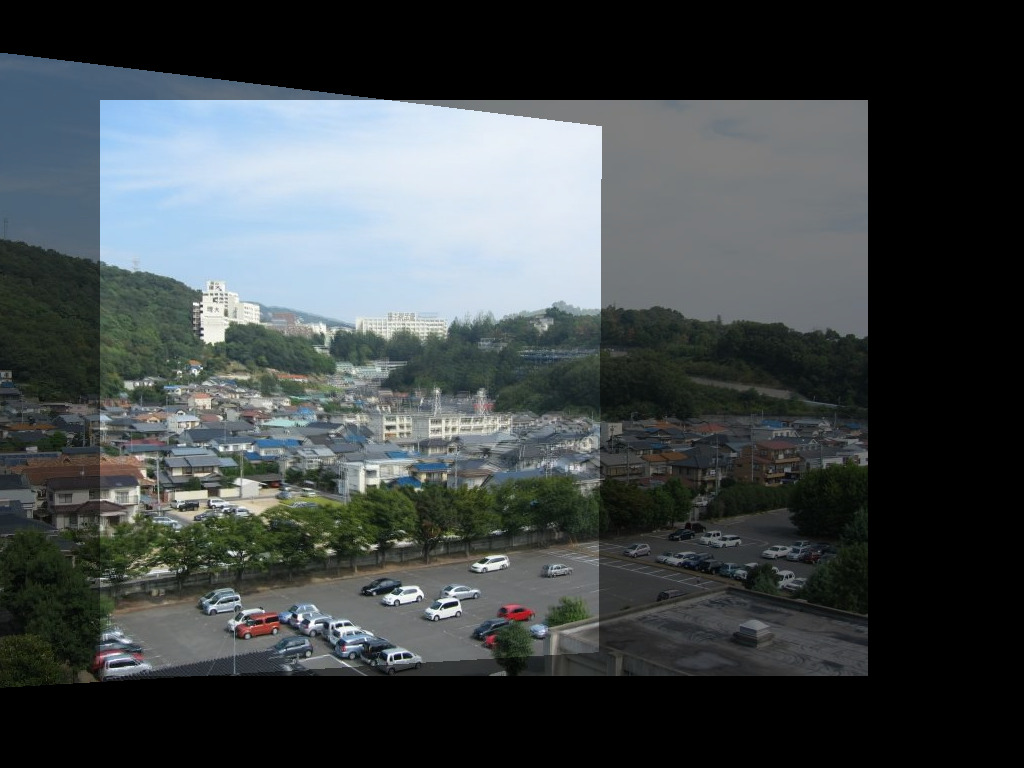
\includegraphics[scale=.3]{dai6.jpg}
        \caption{結果}
    \end{figure}

\section{下記の観点で考察または実装しなさい.}
余力がなかったので行っていない

\section{感想}
難しくてよくわからなかった.資料に合わせてプログラミングをしていただけになったので,
考察もよくかけなかった.今日は理解するまでの時間が足りないなと感じた.

\end{document}
